\documentclass[11pt]{article}

% --------------------------------------------------
% Packages
% --------------------------------------------------
\usepackage[margin=1in]{geometry}
\usepackage{amsmath, amssymb, amsthm}
\usepackage{mathtools}
\usepackage{graphicx}
\usepackage{float}
\usepackage{enumitem}
\usepackage{hyperref}
\usepackage{xcolor}
\usepackage{tikz}
\usetikzlibrary{arrows.meta, positioning, calc}

% Pseudocode and algorithms
\usepackage{algorithm}
\usepackage{algpseudocode}

% Better fonts (optional)
\usepackage{lmodern}

% --------------------------------------------------
% Hyperref setup
% --------------------------------------------------
\hypersetup{
	colorlinks=true,
	linkcolor=blue,
	citecolor=blue,
	urlcolor=blue
}

% --------------------------------------------------
% Theorem-like environments
% --------------------------------------------------
\theoremstyle{definition}
\newtheorem{definition}{Definition}[section]
\newtheorem{theorem}{Theorem}[section]
\newtheorem{claim}{Claim}[section]
\newtheorem{remark}{Remark}[section]

\theoremstyle{proof}
% Proof environment is built-in via amsthm

% --------------------------------------------------
% Custom commands
% --------------------------------------------------
\newcommand{\Gen}{\mathsf{Gen}}
\newcommand{\Enc}{\mathsf{Enc}}
\newcommand{\Dec}{\mathsf{Dec}}
\newcommand{\negl}{\mathsf{negl}}

% --------------------------------------------------
% Document
% --------------------------------------------------
\begin{document}
	
	\title{Public Key Crypto notes - 01}
	\date{February 12. 2026.}
	\author{By contributors}
	\maketitle
	
	% --------------------------------------------------
	\section{Symmetric key crypto recap}
	% --------------------------------------------------

	\begin{itemize}
		\item Symmetric key algorithms, schemes (AES, DES, block ciphers, MACs, etc.)
		\item Given two parties A, B
		\item They have a \emph{shared secret key} $k$
		\item There is an encryption function $Enc_k(m)=c$
		\item And there's also a decryption function $Dec_k(c)=m$
		\item Properties:
		\begin{itemize}
			\item Symmetric: the roles, keys of A and B are symmetric
			\item Fast and efficient encryption \& decryption
		\end{itemize}
	\end{itemize}
	
	% --------------------------------------------------
	\section{Public key (asymmetric) cryptography (PKC)}
	% --------------------------------------------------
	
	\begin{itemize}
		\item Encryptions (RSA, ElGamal, elliptic curve based cryptography)
		\item Digital signatures
		\item Syntax of PKC:
		\begin{itemize}
			\item There are two kinds of keys
			\item $e$ - Encryption key, which is public
			\item $d$ - Decryption key, which is private, kept in secret
		\end{itemize}
		\item $c = Enc_e(m)$
		\item $m = Enc_d(c)$
	\end{itemize}
	
	\subsection{Properties of PKC}
	
	\begin{itemize}
		\item Asymmetric
		\item Slower, computationally more expensive calculations compared to symmetric key cryptography
		\item Since it is so expensive to individually encrypt and decrypt each message in an asymmetrical way, modern ciphersuites often do the following:
		\begin{itemize}
			\item Exchange the shared secret key between two parties using each party's keypairs (e.g. using the Diffie-Hellman key exchange),
			\item Once the shared key is exchanged in an encrypted way over any channel, continue the communication using a symmetric cipher (like AES in GCM mode) and the shared key (which is the same for both parties).
		\end{itemize}
		\item Ralph Merkle: "The inventor of PKC" and commutative encryption.
	\end{itemize}
	
	\begin{definition}[Commutative encryption]
	\[
	\text{An encryption scheme } \Enc_k(\cdot) \text{ is \emph{commutative} if for all messages } m
	\text{ and all keys } k_1, k_2,
	\]
	\[
	\Enc_{k_1}(\Enc_{k_2}(m)) = \Enc_{k_2}(\Enc_{k_1}(m)).
	\]
	
	Equivalently, the order of encryption under different keys does not matter:
	\[
	\Enc_{k_1} \circ \Enc_{k_2} = \Enc_{k_2} \circ \Enc_{k_1}.
	\]
	\end{definition}
	
	\subsection{R. Merkle - exchanging a shared key using a commutative encryption scheme}
	
	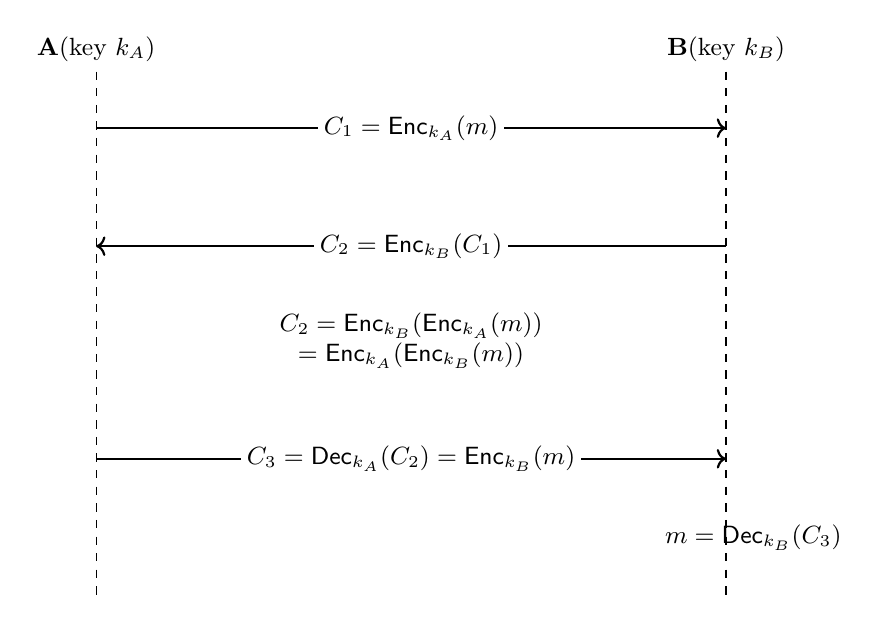
\begin{tikzpicture}[
		font=\small,
		msg/.style={->, thick},
		lab/.style={midway, fill=white, inner sep=2pt}
		]
		
		% Participants
		\node (A) at (0,0) {\textbf{A}\\(key $k_A$)};
		\node (B) at (8,0) {\textbf{B}\\(key $k_B$)};
		
		% Lifelines
		\draw[dashed] (A) -- (0,-7);
		\draw[dashed] (B) -- (8,-7);
		
		% Message 1
		\draw[msg] (0,-1) -- (8,-1)
		node[lab] {$C_1 = \Enc_{k_A}(m)$};
		
		% Message 2
		\draw[msg] (8,-2.5) -- (0,-2.5)
		node[lab] {$C_2 = \Enc_{k_B}(C_1)$};
		
		% Commutativity annotation
		\node[align=center] at (4,-3.7) {
			$C_2 = \Enc_{k_B}(\Enc_{k_A}(m))$\\
			$= \Enc_{k_A}(\Enc_{k_B}(m))$
		};
		
		% Message 3
		\draw[msg] (0,-5.2) -- (8,-5.2)
		node[lab] {$C_3 = \Dec_{k_A}(C_2) = \Enc_{k_B}(m)$};
		
		% Local decryption at B
		\node[align=left] at (8.4,-6.2) {
			$m = \Dec_{k_B}(C_3)$
		};
		
	\end{tikzpicture}
	
	\begin{itemize}
		\item This way, the shared key never gets sent on the insecure channel as a plaintext.
		\item It always travels with at least one layer of encryption.
		\item Let's see if the one-time pad scheme could be used this way.
	\end{itemize}

	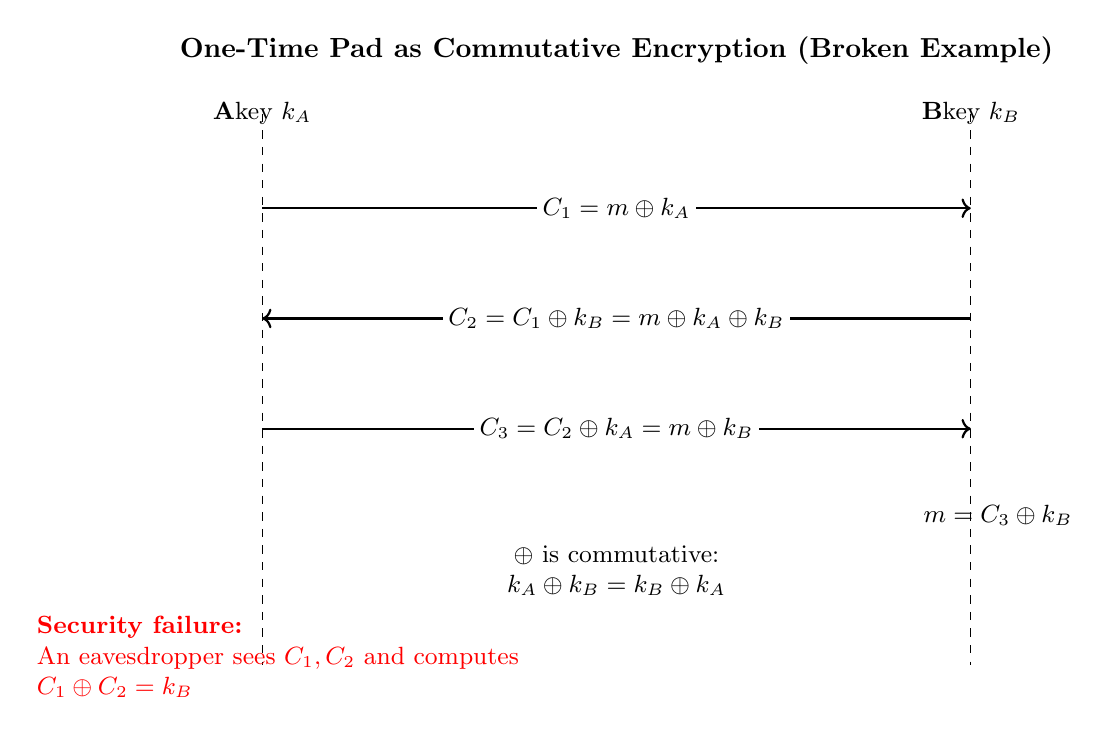
\begin{tikzpicture}[
		font=\small,
		msg/.style={->, thick},
		lab/.style={midway, fill=white, inner sep=2pt}
		]
		
		% Participants
		\node (A) at (0,0) {\textbf{A}\\key $k_A$};
		\node (B) at (9,0) {\textbf{B}\\key $k_B$};
		
		% Lifelines
		\draw[dashed] (0,0) -- (0,-7);
		\draw[dashed] (9,0) -- (9,-7);
		
		% Title
		\node[align=center, font=\bfseries] at (4.5,0.8)
		{One-Time Pad as Commutative Encryption (Broken Example)};
		
		% Message 1
		\draw[msg] (0,-1.2) -- (9,-1.2)
		node[lab] {$C_1 = m \oplus k_A$};
		
		% Message 2
		\draw[msg] (9,-2.6) -- (0,-2.6)
		node[lab] {$C_2 = C_1 \oplus k_B = m \oplus k_A \oplus k_B$};
		
		% Message 3
		\draw[msg] (0,-4.0) -- (9,-4.0)
		node[lab] {$C_3 = C_2 \oplus k_A = m \oplus k_B$};
		
		% Local decryption at B
		\node[align=left] at (9.4,-5.1) {
			$m = C_3 \oplus k_B$
		};
		
		% Commutativity note
		\node[align=center] at (4.5,-5.8) {
			$\oplus$ is commutative: \\
			$k_A \oplus k_B = k_B \oplus k_A$
		};
		
		% Security failure annotation
		\node[align=left, text=red] at (0.2,-6.9) {
			\textbf{Security failure:}\\
			An eavesdropper sees $C_1, C_2$ and computes\\
			$C_1 \oplus C_2 = k_B$
		};
		
	\end{tikzpicture}
	
	\begin{itemize}
		\item The OTP scheme could not be used this way, since B's key would leak in the presence of an eavesdropper.
	\end{itemize}
	
	\subsection{Diffie-Hellman (DH) key exchange}
	
	\begin{itemize}
		\item Whitfeld Diffie and Martin Hellman developed a secure commutative encryption scheme in 1973 and is mainly used as a key exchange protocol.
		\item Take a large prime $p$ and a number $g \pmod{p}$, where $g \in \mathbb{Z}_p$
	\end{itemize}
	
	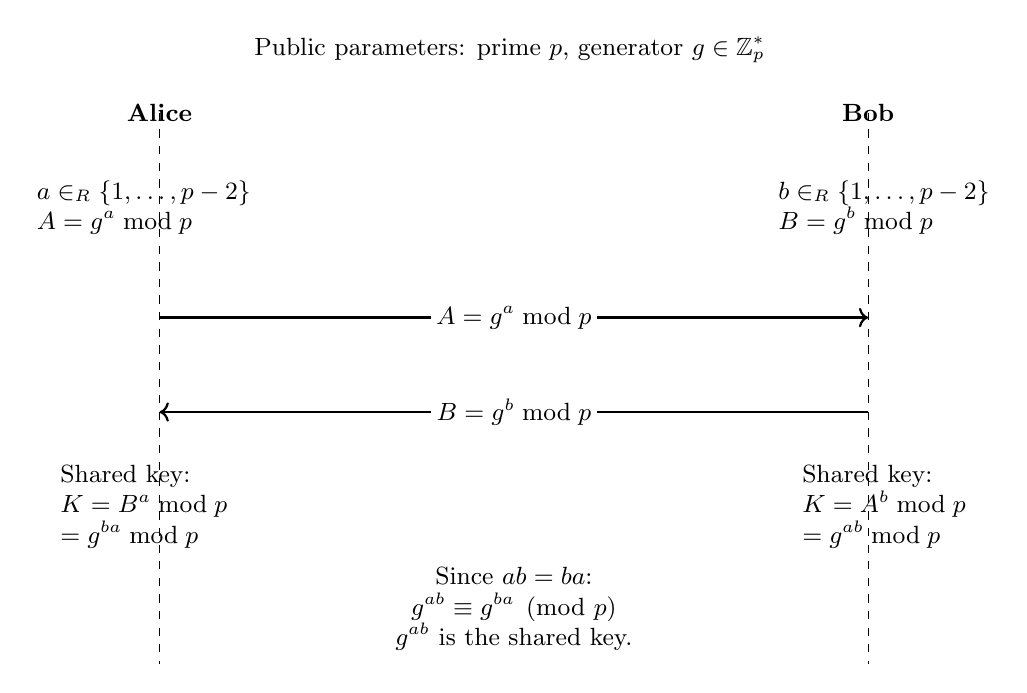
\begin{tikzpicture}[
		font=\small,
		msg/.style={->, thick},
		lab/.style={midway, fill=white, inner sep=2pt}
		]
		
		% Participants
		\node (A) at (0,0) {\textbf{Alice}};
		\node (B) at (9,0) {\textbf{Bob}};
		
		% Lifelines
		\draw[dashed] (0,0) -- (0,-7);
		\draw[dashed] (9,0) -- (9,-7);
		
		% Public parameters
		\node[align=center] at (4.5,0.8) {
			Public parameters: prime $p$, generator $g \in \mathbb{Z}_p^{*}$
		};
		
		% A's local computation
		\node[align=left] at (-0.2,-1.2) {
			$a \in_R \{1,\dots,p-2\}$\\
			$A = g^a \bmod p$
		};
		
		% B's local computation
		\node[align=left] at (9.2,-1.2) {
			$b \in_R \{1,\dots,p-2\}$\\
			$B = g^b \bmod p$
		};
		
		% Message A -> B
		\draw[msg] (0,-2.6) -- (9,-2.6)
		node[lab] {$A = g^a \bmod p$};
		
		% Message B -> A
		\draw[msg] (9,-3.8) -- (0,-3.8)
		node[lab] {$B = g^b \bmod p$};
		
		% Shared key computation A
		\node[align=left] at (-0.2,-5.0) {
			Shared key:\\
			$K = B^a \bmod p$\\
			$= g^{ba} \bmod p$
		};
		
		% Shared key computation B
		\node[align=left] at (9.2,-5.0) {
			Shared key:\\
			$K = A^b \bmod p$\\
			$= g^{ab} \bmod p$
		};
		
		% Equality annotation
		\node[align=center] at (4.5,-6.3) {
			Since $ab = ba$:\\
			$g^{ab} \equiv g^{ba} \pmod p$\\
			$g^{ab}$ is the shared key.
		};
		
	\end{tikzpicture}
	
	\begin{itemize}
		\item If $a$ can be computed from $g^a$. then this key exchange protocol would be breakable.
		\item This problem is the \emph{Discrete logarithm problem}, which is computationally hard.
		\item Questions:
			\item Is the Discrete logarithm problem really hard?
			\item What is the generator number $g$? How can we choose it?
			\item How large would $p$ need to be?
	\end{itemize}
	
	\section{Number theoretic backgrounds}
	
	\begin{definition}[Order of the generator]
		Let $p$ be a prime number and $g \in \mathbb{Z}_p, g \ne 0$. Then, the order of $g$ ($ord_p g$) is the smallest $k \le 1$, such that:
		$$
		g^k \equiv 1 \pmod{p}
		$$
	\end{definition}
	
	\begin{remark}
		This is well-defined by Fermat's little theorem: $g^{p-1} \equiv 1 \pmod{p}$.
	\end{remark}
	
	\begin{remark}
		$ord_p g$: The order of $g$ is the number of possible powers of $g$ modulo $p$.
	\end{remark}
	
	\begin{align}
		g^0 = 1;g^1 = g; g^2; g^3; \dots g^{ord_p(g)-1} \\
		g^{ord_p(g)} = 1; g^{ord_p(g)+1} = 1 \cdot g = g 
	\end{align}
	
	\begin{claim}
		$ord_p(g) | p-1$ ($ord_p(g)$ divides $p-1$)
	\end{claim}
	\begin{proof}
		Let $\sigma = ord_p (g)$
		\begin{align}
			p-1 = \sigma \cdot q + r && 0 \le r \le \sigma \\
			1 = g^{p-1} = g^{\sigma \cdot q + r} = && \text{(by Fermat's little theorem)} \\
			= (g^{\sigma})^q \cdot g^r && \text{(where $g^\sigma$ comes from the definition of the order of $g$)}
		\end{align}
		i.e.: $1=g^r$ by the minimality of the $ord$, $r=0$
	\end{proof}
	
	\begin{definition}[generator]
		Let $p$ be a prime and $g \in \mathbb{Z}_p, g \ne 0$. Then $g$ is a generator if:
		$$
		ord_p(g) = p-1
		$$
	\end{definition}
	
	\begin{remark}
		One can prove that there are always generators.
	\end{remark}
	
	\begin{theorem}
		Let $p$ be a prime and write $p-1 = q_1^{e_1} \cdot q_2^{e_2} \cdot \dots \cdot q_t^{e_t}$.
		Then $g$ is a generator if and only if:
		$$
		g^{\frac{p-1}{q_i}} \equiv 1 \pmod{p}
		$$
		for all $i$.
	\end{theorem}
	
	\begin{proof}
		Prove from left-to-right: We know that $g$ is a generator. Then:
		$$
		ord_p(g) = p-1
		$$
		So, by the minimality of the $ord$, $g^{\frac{p-1}{q_i}} \not\equiv 1 \pmod{p}$.
		
		Prove from right-to-left: Suppose that $g$ is \emph{not} a generator, i.e.: $g^k \equiv 1 \pmod{p}$, $1 \le k < p-1$.
		As $k | p-1$, write $p-1 = s \cdot k$.
		Let $q_i | s$, then:
		$$
		g^{\frac{p-1}{q_i}} = g^{\frac{s \cdot k}{q_i}} = g^{\frac{s}{q_i} \cdot k} = (g^k)^{\frac{s}{q}} = 1
		$$
	\end{proof}
	
	\begin{remark}
		Typical choice for $p$ is $p = 2q + 1$, where $q$ is a prime. Here, $p$ is called a "safe" prime, while $q$ is called a "Sophie Germain prime".\footnote{\url{https://en.wikipedia.org/wiki/Safe_and_Sophie_Germain_primes}}
	\end{remark}
	
\end{document}
